\documentclass{beamer}
%\usepackage[all,arc,curve,frame,color]{xy}
%\usepackage{tkz-graph}
\usepackage{mathtools}
\usepackage{ragged2e,etoolbox}


\newenvironment{nstabbing}
  {\setlength{\topsep}{0pt}%
   \setlength{\partopsep}{0pt}%
   \tabbing}
  {\endtabbing}

\def\jump{ \quad \\ \vspace{0.7cm} \pause}
\newcommand{\nc}{\newcommand}
\nc{\pid}{\mathfrak{p} }
\nc{\dpid}{\delta_{\mathfrak{p}}}

\def\AA{{\mathbb A}}
\def\CC{{\mathbb C}}
\def\EE{{\mathcal E}}
\def\FF{{\mathcal F}}
\def\GG{{\mathcal G}}
\def\HH{{\mathcal H}}
\def\MM{{\mathcal M}}
\def\NN{{\mathbb N}}
\def\PP{{\mathbb P}}
\def\QQ{{\mathbb Q}}
\def\RR{{\mathbb R}}
\def\ZZ{{\mathbb Z}}
\def\aa{{\mathbf a}}
\def\bb{{\mathbf b}}
\def\del{\partial}
\def\kk{\Bbbk}
\def\mm{{\mathfrak m}}
\def\nn{{\mathfrak n}}
\def\pp{{\mathfrak p}}
\def\qq{{\mathfrak q}}
\def\rr{{\mathbf r}}
\def\uu{{\mathbf u}}
\def\vv{{\mathbf v}}
\def\ww{{\mathbf w}}
\def\xx{{\mathbf x}}
\def\yy{{\mathbf y}}
\def\zz{{\mathbf z}}
\newcommand{\PGL}{\textrm{PGL}}
\newcommand{\res}{\textrm{Res}}


\DeclareMathOperator{\Tail}{Tail}
\DeclareMathOperator{\Per}{Per}
\DeclareMathOperator{\PrePer}{PrePer}
\DeclareMathOperator{\HTail}{HTail}
\DeclareMathOperator{\HPer}{HPer}
\DeclareMathOperator{\HPrePer}{HPrePer}

\makeatletter
\def\th@mystyle{%
    \normalfont % body font
    \setbeamercolor{block title example}{bg=orange,fg=white}
    \setbeamercolor{block body example}{bg=orange!20,fg=black}
    \def\inserttheoremblockenv{exampleblock}
  }
\makeatother

\makeatletter
\def\th@thmstyle{%
    \normalfont % body font
    \setbeamercolor{block title example}{bg=blue,fg=white}
    \setbeamercolor{block body example}{bg=blue!20,fg=black}
    \def\inserttheoremblockenv{exampleblock}
  }
\makeatother

\definecolor{darkgreen}{RGB}{77,153,0}
\makeatletter
\def\th@qstnstyle{%
    \normalfont % body font
    \setbeamercolor{block title example}{bg=darkgreen,fg=white}
    \setbeamercolor{block body example}{bg=green!20,fg=black}
    \def\inserttheoremblockenv{exampleblock}
  }
\makeatother

\theoremstyle{thmstyle}
\newtheorem*{mydef}{Definition}

\theoremstyle{thmstyle}
\newtheorem*{mythm}{Theorem}

\theoremstyle{mystyle}
\newtheorem*{remark}{Remark}
\newtheorem*{conjecture}{Conjecture}
\newtheorem*{mycor}{Corollary}
\newtheorem*{mylemma}{Lemma}

\theoremstyle{qstnstyle}
\newtheorem*{question}{Question}

\usepackage{remreset}% tiny package containing just the \@removefromreset command
\makeatletter
\@removefromreset{subsection}{section}
\makeatother
\setcounter{subsection}{1}

\newcommand\Wider[2][3em]{%
\makebox[\linewidth][c]{%
  \begin{minipage}{\dimexpr\textwidth+#1\relax}
  \raggedright#2
  \end{minipage}%
  }%
}

\mode<presentation>{\usetheme{CambridgeUS}\usecolortheme{dolphin}} 
%\setbeamertemplate{navigation symbols}{}
\setbeamertemplate{blocks}[rounded][shadow=false]


\title[Bounds for Preperiodic Points]{Bounds for Preperiodic Points for Maps with Good Reduction}
%\subtitle[Dissertation Defense]{Dissertation Defense}
\author[S. Troncoso]{Sebastian Troncoso}
\institute[BSC]{Birmingham-Southern College}
%\titlegraphic{\includegraphics[height=1.5cm]{../images/normale_pisa.png}}
\date[September 15, 2017.]{ September 15, 2017. \\ \vspace{1cm} }


%\AtBeginSection[]{} % for optional outline or other recurrent slide
\AtBeginSection{\frame{\sectionpage}}
\begin{document}

\begin{frame}
\titlepage
\end{frame}

\begin{frame}
\frametitle{Notation}
Let $K$ be a number field \emph{i.e.} $[K: \mathbb{Q}] < \infty$,   
\jump
$\mathbb{Q}$ \quad $\mathbb{Q}(i)$ \quad $\mathbb{Q}(\sqrt{2})$ 
\jump
and $\mathcal{O}_K$ its ring of algebraic integers,
\jump
$\mathbb{Z}$ \quad $\mathbb{Z}(i)$ \quad $\mathbb{Z}(\sqrt{2}).$ 
\jump
Let $\displaystyle \mathbb{P}^1(K)=\{[x:y] \mid  [x:y]\sim [\lambda x:\lambda y] \quad \lambda\in K^{*} \} = K\cup \{\infty \}$ be  the projective line. \pause When we write $\PP^1$ is assume to be $\PP^1(\bar{K})$.

\end{frame}

\begin{frame}
\frametitle{Notation}
$\phi:\mathbb{P}^1\to\mathbb{P}^1$ be an endomorphism defined over $K$.
\jump
$\phi([x:y])=[F(x,y):G(x,y)]$ where $F$ and $G$ are polynomials of the same degree with coefficients in $K$ and with no common zeros.
\jump
$\displaystyle\phi(x)=\frac{f(x)}{g(x)}$ where $f$ and $g$ are polynomials with coefficients in $K$.
\jump
$\phi^n$ is the $n$th iterate of $\phi$.
\\ \pause
The \textbf{orbit} of a point $P\in\PP^1$ is the set 
$$ O_{\phi}(P) = \{P, \phi(P),\phi^2(P),\phi^3(P),\ldots \}.$$

\pause The \textbf{orbit length} of $P$ is the cardinality of the orbit of $P$ (as a set).
\end{frame}

\begin{frame}
\frametitle{Notation}

\textbf{Periodic point}: $\phi^n(P)=P$ for some $n\geq{1}$.
\\\quad\quad \pause Minimal $n$ is called the \textbf{period} of $P$.

\pause
\vspace{2mm}
The set of $K$-rational periodic points for $\phi$ is denoted by $\Per(\phi,K)$.
\\\quad\\
\pause
\textbf{Preperiodic point}: $\exists m\geq{0}$ such that $\phi^m(P)$
is periodic \\\quad\quad \pause \emph{i.e.}  $P$ has finite orbit.

\pause
\vspace{2mm}
The set of $K$-rational preperiodic points for $\phi$ is denoted by $\PrePer(\phi,K)$.
\\\quad\\
\pause
\textbf{Tail point}: A point that is preperiodic but not periodic.

\pause
\vspace{2mm}
The set of $K$-rational tail points for $\phi$ is denoted by $\Tail(\phi,K)$.
\end{frame}

\begin{frame}
\frametitle{Examples:}
We can view $\PP^1(K)$ as $K\cup \{\infty \}$ and endomorphism of $\PP^1$ as rational functions. Consider $\phi_c(z)=z^2+c$.
\pause

\begin{center}
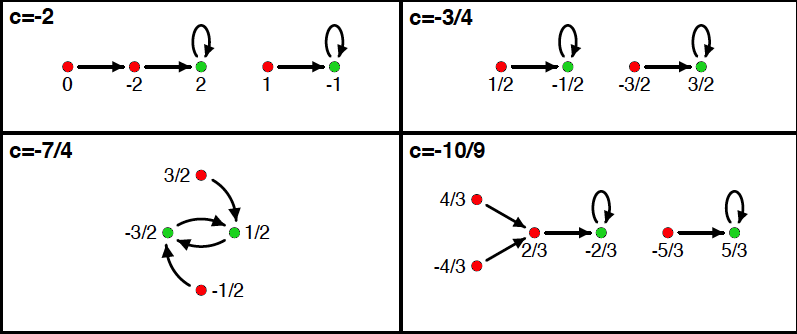
\includegraphics[width=1.0\linewidth]{placeholder4}
\end{center}

$\QQ$-rational tail points (red) and $\QQ$-rational periodic points (green) of  $\phi_c(z)=z^2+c$.
\end{frame}

\begin{frame}
\frametitle{Question:}
\begin{itemize}
\item Are the sets $\Tail(\phi,K)$, $\Per(\phi,K)$ and $\PrePer(\phi,K)$ finite? 

\pause \textbf{Yes}. 
\vspace{6mm}\pause

\begin{mythm}[Northcott 1950]
Let $\phi : \PP^n \to \PP^n$ be an endomorphism of degree $\geq{2}$
defined over a number field $K$. Then $\phi$ has
only finitely many preperiodic points in $\PP^n(K)$.
\end{mythm}

\vspace{6mm} \pause
We can deduce from the original proof of Northcott's theorem  a bound for $|\PrePer(\phi,K)|$ depending on
\begin{itemize}
\item $n$
\item $[K:\QQ]$
\item the degree of $\phi$
\item height of the coefficients of $\phi$
\end{itemize}

 
\end{itemize}
\end{frame}

\begin{frame}
\frametitle{Goals:}
Give explicit bounds for $|\Tail(\phi,K)|$, $|\Per(\phi,K)|$ and $|\PrePer(\phi,K)|$ in terms of:\pause
\begin{itemize}
\item  $D=[K: \QQ]$\pause 

\item The dimension $n$ of the projective space \pause 

\item The degree $d$ of $\phi$.
\end{itemize}

\pause

\begin{conjecture}[Uniform Boundedness Conjecture - Morton--Silverman
  1994]
There exists a bound $B = B(D,n,d)$ such that if $K/\mathbb{Q}$ is a number field of degree $D$, and $\phi:\mathbb{P}^n\rightarrow\mathbb{P}^n$ is an endomorphism of degree $d\geq{2}$ defined over $K$, then 
$$|\text{PrePer}(\phi,K)| \leq B.$$
\end{conjecture}
\end{frame}

\begin{frame}
The conjecture Uniform Boundedness Conjecture (UBC) is an extremely strong uniformity conjecture.
\jump
\begin{itemize}
\item The UBC on maps of degree $4$ on $\PP^1$ defined over $\QQ$ implies Mazur's theorem that the rational torsion subgroup of
an elliptic curve $E/\QQ$ is bounded independently of $E$.
\jump
\item The UBC for maps of degree $4$ on $\PP^1$ defined over $K$ implies Merel's theorem that the size of the rational torsion subgroup
of an elliptic curve over a number field $K$ is bounded only in terms of the degree of $[K : \QQ]$.
\jump
\item  Lattes maps are the only nontrivial family of rational maps for which the UBC is currently known.
\end{itemize}


\end{frame}


\begin{frame}
\frametitle{Poonen's Conjecture}

After Lattes maps the simplest case we could consider for the UBC is \pause  $\phi$ a quadratic polynomial in one variable with coefficients in $\QQ$ and $K=\QQ$.

\pause
\vspace{4mm}


\begin{conjecture}[Poonen's Conjecture]
Let $\phi$ be a quadratic polynomial defined over $\mathbb{Q}$ then 
$$|\PrePer(\phi,\QQ)| \leq 9.$$
\end{conjecture}

\pause
\vspace{6mm}

If $\phi=x^2+d$ then B. Hutz and P. Ingram have shown that Poonen's conjecture holds when the numerator and denominator of $d$ don't exceed $10^8$.

\end{frame}

\begin{frame}
\frametitle{Goals:}

In order to get explicit bounds for the cardinality of the set $\PrePer(\phi,K)$ we need an extra parameter. 

Instead of the height of $\phi$ we can use a weaker and more natural parameter to get bound on $|\PrePer(\phi,K)|$.\pause 
\jump
This parameter is the number of places of bad reduction of $\phi$.
\jump
Give explicit bounds for $|\Tail(\phi,K)|$, $|\Per(\phi,K)|$ and $|\PrePer(\phi,K)|$ in terms of:
\begin{itemize}
\item  $D=[K: \QQ]$ 

\item The dimension $n$ of the projective space  

\item The degree $d$ of $\phi$.

\item The number of places of bad reduction of $\phi$.
\end{itemize}


\end{frame}

\begin{frame}
\frametitle{Normalized Form and Good Reduction}
Let $\phi$ be an endomorphism of $\PP^1$ defined over $K$, $\mathfrak{p}$ be a non zero prime ideal of $\mathcal{O}_K$
, $\mathcal{O}_{\mathfrak{p}}$ the local ring at $\pid$ and $k=\mathcal{O}_{\mathfrak{p}}/\pid$ the residue field of $\mathcal{O}_{\mathfrak{p}}$. Let $F,G \in K[X,Y]$ be homogeneous polynomials of the same degree with no common zero on $\PP^1$ \jump


\begin{itemize}
\item We say that $\phi=[F, G]$ is in  \textbf{normalized form} with respect to $\pid$ if  all the coefficients of $F,G$ are in $\mathcal{O}_\pid$ and at least one is a $\pid$-unit. \jump
\item For an any representation $\phi=[F, G]$ we can find a $c\in K^{*}$ such that $[cF,cG]$ is in normalized form with respect to $\pid$.
\end{itemize}
\end{frame}

\begin{frame}
\frametitle{Normalized Form and Good Reduction}

\begin{itemize}
\item Write $\phi=[F, G]$ in normalized form with respect to $\pid$. Consider the reduction of $\phi$ modulo $\pid$ given by
$$\tilde{\phi}=[\tilde{F},\tilde{G}] $$
In other words, $\tilde{\phi}$ is obtained by reducing the coefficients of $F,G$ modulo $\pid$.
\jump
Then $\phi$ has \textbf{good reduction} at $\pid$ if the system of equations $\tilde{F}=\tilde{G}=0$ have no common zero in $\mathbb{P}^1(\bar{k})$.

\jump
\item $\phi$ has \textbf{bad reduction} at $\pid$ if it does not have good reduction at $\pid$.
\end{itemize}
\end{frame}

\begin{frame}
\frametitle{Normalized Form and Good Reduction}
Let $S$ be a finite set of places $K$, including all archimedean ones. \pause We recall that there is a bijection between non archimedean places and primes of $\mathcal{O}_K$.
\jump
\begin{itemize}
\item We say that $\phi$  has \textbf{good reduction outside} $S$ if $\phi$ has good reduction for every $\pid \notin S$.

\jump
\end{itemize}

If we allow the number of primes of bad reduction as a parameter, much more is known for the cardinality of the set of $K$-rational preperiodic points. 
\end{frame}



\begin{frame}
\frametitle{Bound on maximal period}
\begin{mythm}[W.\ Narkiewicz 1988]
Let $\phi \in K[z]$ be a polynomial of degree $\geq{2}$
defined over a number field $K$ of degree $D=[K:\QQ]$. 
Suppose $\phi$ has good reduction outside a finite set of places $S$, including all archimedean ones. Let $s=|S|$.
\\\quad\\
If $P$ is a $K$-rational periodic point of period $n$, then
$$ n \leq (6\cdot 7^{D+2s})^\alpha,$$ where $\alpha=O(s\log{s}).$
\end{mythm}
\end{frame}




\begin{frame}
\frametitle{Bound on maximal orbit length of a preperiodic point}
\begin{mythm}[J.K.\ Canci 2006]
Let $\phi : \PP^1\to\PP^1$ be a rational map of degree at least two
defined over a number field $K$. 
Suppose $\phi$ has good reduction outside a finite set of places $S$, including all archimedean ones. Let $s=|S|$.
\\\quad\\
If $P\in\text{PrePer}(\phi,K)$ is of orbit length $n$, then
$$n\leq\left[{e^{10}}^{12}(s+1)^8(log(5(s+1)))^8\right]^s.$$
\end{mythm}
\end{frame}

\begin{frame}
\frametitle{Bound on maximal orbit length of a preperiodic point }
\begin{mythm}[J.K.\ Canci, L.\ Paladino 2015]
Let $\phi : \PP^1\to\PP^1$ be a rational map of degree $\geq{2}$
defined over a number field $K$ and $[K: \mathbb{Q}]=D$. 
Suppose $\phi$ has good reduction outside a finite set of places $S$, including all archimedean ones. Let $s=|S|$.
If $P\in\text{PrePer}(\phi,K)$ is of orbit length $n$, then
$$n\leq \max\left\{(2^{16s-8}+3)\left[12s\log(5s)\right]^{D}, \left[12(s+2)\log(5s+5)\right]^{4D}\right\}
.$$
\end{mythm}
\jump
From here we can deduce a bound for $|\PrePer(\phi,K)| $ that is roughly of the order $\displaystyle d^{2^{16s}\left( s\log(s) \right)^{D}}$.

\end{frame}




%\begin{frame}
%\frametitle{From bound of maximal period to bound of $\#\text{Per}(\phi,K)$}
%
%\begin{remark}
%
%Given a bound on the maximal period of a $K$-rational periodic point, we can get a (naive) bound on the number of periodic points, as any periodic point of period $\leq{N}$ satisfies some equation $f^n(P)=P$ for $1\leq{n}\leq{N}$.
%
%\quad \\
%
%We can get in this way a bound that is on the order of $O(d^N)$, where $N$ is the maximal possible period.
%\end{remark}
%\end{frame}

%\begin{frame}
%\frametitle{Best \textbf{full} bound (so far) for polynomials}
%\begin{mythm}[R.L.\ Benedetto 2007]
%Let $\phi \in K[z]$ be a polynomial of degree $d\geq{2}$
%defined over a number field $K$ of degree $D=[K:\QQ]$. 
%Suppose $\phi$ has good reduction outside a finite set of places $S$, including all archimedean ones. Let $s=|S|$.
%The number of preperiodic points of $\phi$ in $\PP^1(K)$ is at most $O(s\log s)$ and $O(d^2/\log{d})$. 
%\end{mythm}
%
%\pause
%
%\begin{itemize}
%\item Proved by using nonarchimedean places $\nu$ of bad reduction and bounding the filled Julia set in the completion $K_\nu$.  \pause
%\item X.\ Faber (2015) used ``Benedetto's trick'' to find exact number of preperiodic points in certain infinite sequences of quadratic polynomials.
%\end{itemize}
%\end{frame}





\begin{frame}
\frametitle{Bounds independent of the degree}
\begin{mythm}[S.\ Troncoso 2016]
Let $K$ be a number field and $S$ a finite set of places of $K$ containing all the archimedean ones. Let $\phi $ be an endomorphism of $\PP^1$, defined over $K$, and $d \geq 2$ the degree of $\phi$. Assume $\phi$ has  good reduction outside $S$.
\begin{enumerate}

\item [(a)] 
If there are at least three $K$-rational tail points of $\phi$ then
$$|\Per(\phi,K)| \leq 2^{16|S|}+3. $$

\item [(b)]
If there are at least four $K$-rational periodic points of $\phi$ then
$$|\Tail(\phi,K)| \leq 4(2^{16|S|}).$$
\end{enumerate}
\end{mythm}
\pause
Notice that under these hypotheses the bounds are independent of the degree of $\phi$. Those hypotheses are sharp, \emph{i.e.} if there are two (three) $K$-rational tail (periodic) points then $|\Per(\phi,K)|$ ($|\Tail(\phi,K)|$) must depend on $d$. 
\end{frame}

\begin{frame}
\frametitle{Bounds for Preperiodic points}

Using  some important results from the theory:\pause
\begin{itemize}
\item Riemann-Hurwitz formula
\jump
\item  Baker's Theorem on existence of periodic points
\jump
\item Kisaka's analysis on Baker's Theorem
\end{itemize}
\jump We can prove an explicit bound for the desire sets.

\end{frame}

\begin{frame}
\begin{mythm}[S.\ Troncoso 2016]
Let $K$ be a number field and $S$ a finite set of places of $K$ containing all the archimedean ones. Let $\phi $ be an endomorphism of $\PP^1$, defined over $K$, and $d \geq 2$ the degree of $\phi$. Assume $\phi$ has  good reduction outside $S$. Then
\begin{enumerate}
\item [(a)] $|\Per(\phi,K)| \leq  2^{16|S|d^3}+3.$

\item [(b)] $|\Tail(\phi,K)| \leq  4(2^{16|S|d^3}) .$

\item [(c)] $|\PrePer(\phi,K)| \leq 5(2^{16|S|d^3})+3.$

\end{enumerate}
\end{mythm}

Notice that the bounds obtained  in the theorem are a significant improvement from the previous bound given by Canci and Paladino which was of the order $\displaystyle d^{2^{16s}\left( s\log(s) \right)^{D}}$ for the set $|\PrePer(\phi,K)|$.

\end{frame}

\begin{frame}
\frametitle{Bounds independent of the degree}
\begin{mythm}[S.\ Troncoso 2016]
Let $K$ be a number field and $S$ a finite set of places of $K$ containing all the archimedean ones. Let $\phi $ be an endomorphism of $\PP^1$, defined over $K$, and $d \geq 2$ the degree of $\phi$. Assume $\phi$ has  good reduction outside $S$.
\begin{enumerate}

\item [(a)] 
If there are at least three $K$-rational tail points of $\phi$ then
$$|\Per(\phi,K)| \leq 2^{16|S|}+3. $$

\item [(b)]
If there are at least four $K$-rational periodic points of $\phi$ then
$$|\Tail(\phi,K)| \leq 4(2^{16|S|}).$$
\end{enumerate}
\end{mythm}
\end{frame}


\begin{frame}
\frametitle{Tools}
Before to prove our theorem we need to introduce three tools:\jump
\begin{itemize}
\item Logarithmic $p$-adic chordal distance.

\jump

\item $S$-unit equation.

\jump

\item Study the distance between periodic and tail points.
\end{itemize}

\end{frame}


\begin{frame}
\frametitle{logarithmic $p$-adic chordal distance}

Let $K$ be a number field, and $\nu_{\pid}$ a valuation associated to a prime $\pid$ of $K$. 
\quad \\ 

Let $P=[X_1:Y_1], Q=[X_2:Y_2] \in \PP^1(K)$. Then

\quad \\ \pause
\textbf{logarithmic $p$-adic chordal distance}:

$$\delta_{\mathfrak{p}}\,(P,Q)=v_{\mathfrak{p}}\,(X_1Y_2-X_2Y_1)-\min\{v_{\mathfrak{p}}(X_1),v_{\mathfrak{p}}(Y_1)\}-\min\{v_{\mathfrak{p}}(X_2),v_{\mathfrak{p}}(Y_2)\}$$
\end{frame}

%\begin{frame}
%\frametitle{$S$-integral points}
%
%\begin{itemize}
%\item Let $P,Q \in \PP^1(K)$. Then $P\equiv{Q}\pmod{\pid}$ iff $\delta_\pid(P,Q)\geq{1}$. \jump
%\item Let $S$ be a finite set of places of $K$ containing all the archimedean ones. \jump
%\item $P$ is \textbf{$S$-integral} with respect to $Q$ iff $\delta_\pid(P,Q)=0$ for all $\pid\not\in{S}$. \jump
%% \item A finite point $P$ is an $S$-integer iff it is $S$-integral with respect to $\infty$.
%\end{itemize}
%\end{frame}


\begin{frame}
\frametitle{$S$-unit equations}
Let $S$ be a finite set of places of $K$ containing all the archimedean ones and $\mathcal{O}_S^{*}$ be the group of $S$-units of $\mathcal{O}_K$.\pause

\begin{itemize}

\item A linear relation of the form $$au+bv=1$$  where  $(u,v) \in \left(\mathcal{O}_S^*\right)^2$ and $a,b\in K^{*}$ is called a $S$-unit equation. \pause
\item Beukers and Schlickewei give an explicit bound  for the $S$-unit equation. The number of solutions $(u,v) \in \left(\mathcal{O}_S^{*}\right)^2$ to 
$$au+bv=1$$ 
is bounded by $$2^{8(2|S|+2)}.$$
\end{itemize}
\end{frame}



\begin{frame}
\frametitle{Distance between periodic and tail points}
\begin{mythm}[S.\ Troncoso 2016]
Let $\phi$ be an endomorphism of $\PP^1$, defined over $K$. Suppose $\phi$ has good reduction outside $S$. Let $R\in\PP^1(K)$ be a tail point and let $n$ be the period of the periodic part of the orbit of $R$. Let $P\in\PP^1(K)$ be any periodic point that is not $\phi^{mn}(R)$ for some $m$. Then $\delta_\pp(P,R)=0$ for every $\pp \notin S$.
\end{mythm}

For simplicity suppose $\mathcal{O}_S$ is a PID and write $P=[x:y]$ and $Q=[w:t]$ in coprime $S$-integer coordinates.

\pause Using the theorem we get that there is a $S$-unit element $u$ such that
$$xt-yw=u $$

 
\end{frame}

%\begin{frame}
%\frametitle{Bounds independent of the degree}
%
%\begin{mythm}[S.\ Troncoso 2016]
%Let $K$ be a number field and $S$ a finite set of places of $K$ containing all the archimedean ones. Let $\phi $ be an endomorphism of $\PP^1$, defined over $K$, and $d \geq 2$ the degree of $\phi$. Assume $\phi$ has  good reduction outside $S$.
%\begin{enumerate}
%
%\item [(a)] \label{th 3 periodic}
%If there are at least three $K$-rational tail points of $\phi$ then
%$$|\Per(\phi,K)| \leq 2^{16|S|}+3. $$
%
%\item [(b)] \label{th 4 preperiodic}
%If there are at least four $K$-rational periodic points of $\phi$ then
%$$|\Tail(\phi,K)| \leq 4(2^{16|S|}).$$
%\end{enumerate}
%\end{mythm}
%Lets prove part $(a)$ of this theorem.
%\end{frame}
%
%
%
%\begin{frame}
%\frametitle{Proof of (a):}
%
%For simplicity we assume that $\mathcal{O}_S$ is a PID. \pause Let $P_1,P_2,P_3$ be three different $K$-rational tail points and $n_i$ be the period of the periodic part of $P_i$.\jump
%
%Let $P$ be a $K$-rational periodic point such that $\phi^{mn_i}(P_i)\neq  P$ for $1\leq i \leq 3$ and every $m>0$. \pause Write $P=[x:y]$ and $P_i=[x_i:y_i]$ in coprime $S$-integer coordinates.\jump Using the arithmetic relation between $K$-rational tail points and $K$-rational periodic points we get the systems of equations 
%$$x_1y-y_1x=u_1 $$
%$$x_2y-y_2x=u_2 $$
%$$x_3y-y_3x=u_3$$ 
%for $u_1,u_2,u_3 \in\mathcal{O}_S^{*}$ 
%\end{frame}
%
%\begin{frame}
%\frametitle{Proof of (a):}
%
%Solving for $x$ and $y$ we get the $S$-unit equation
%$$A\frac{u_1}{u_3}+B\frac{u_2}{u_3}=1. $$
%
%\pause We know that this system has at most $2^{16s+16}$ solutions.\jump
%
%Finally, $P=[x:y]=[\frac{x}{y}:1]$ and $\frac{x}{y}$ can be express in terms of $x_1,y_1,x_3,y_3,\frac{u_1}{u_3}$. We conclude that
%
%$$|\Per(\phi,K)| \leq 2^{16s+16}+3. $$
%\end{frame}

\begin{frame}
\frametitle{Another technique}

Using another technique we can get a better result in terms of $d$. \pause

\begin{mythm}[S.\ Troncoso 2017]
Let $K$ be a number field and $S$ a finite set of places of $K$ containing all the archimedean ones. Let $\phi $ be an endomorphism of $\PP^1$, defined over $K$, and $d \geq 2$ the degree of $\phi$. Assume $\phi$ has  good reduction outside $S$. Then

\begin{enumerate}

\item [(a)] $|\Tail(\phi,K) | \leq d\max\left\{  (5 \cdot 10^6 (d^3+1))^{|S|+4} ,4(2^{64(|S|+3)}) \right \}.$\jump

\item [(b)] In addition, if $\phi$ has at least one $K$-rational tail point then then
$$|\Per(\phi,K)| \leq   \max \left\{  (5 \cdot 10^6 (d-1))^{|S|+3} ,4(2^{128(|S|+2)}) \right\}+1.$$
\end{enumerate}
\end{mythm}

\pause


The proof of this theorem uses all the techniques mentions before. But it uses Thue Mahler equations instead of using $S$-unit equations.
\end{frame}




\begin{frame}
\frametitle{Another technique: Thue-Mahler equations}
Let $F(X,Y)$ be a binary  form of degree $r \geq 3$ with coefficients in $\mathcal{O}_S$  which is irreducible over $K$.\jump  An $\mathcal{O}_S^{*}$-coset of solutions of
\begin{equation} \label{T-M}
 F(x,y) \in \mathcal{O}_S^{*}  \quad\quad \mbox{ in } \quad (x,y) \in \mathcal{O}_S^{2}
\end{equation}
is a set $\{\epsilon(x,y): \epsilon \in \mathcal{O}_S^{*} \}$, where $(x,y)$ is a fixed solution of (\ref{T-M}).
\jump

Evertse proved in 1997 that: the set of solutions of (\ref{T-M}) is the union of at most
$$ (5\cdot 10^6r)^s$$
$\mathcal{O}_S^{*}$-cosets of solutions.
\end{frame}




\begin{frame}
\frametitle{Almost ready project}
Joint work with J.K.\ Canci and S.\ Vishkautsan \\
\pause
\begin{mythm}[S.\ Troncoso 2016]
Let $K$ be a number field and $S$ a finite set of places of $K$ containing all the archimedean ones. 
Let $\phi$ be an endomorphism of $\PP^1$, defined over $K$, and $d\geq 2$ the degree of $\phi$. Assume $\phi$ has good reduction outside $S$. Then 
$$|{\rm PrePer}(\phi,K)| \leq \kappa_1 d^2+\lambda_1$$

If we assume that $\phi$ has a $K$-rational periodic point of minimal period at least two then
$$|{\rm PrePer}(\phi,K)| \leq \kappa_2 d+\lambda_2.$$
\end{mythm}
\pause 

We emphasize that the constants $\kappa_1,\kappa_2,\lambda_1$ and $\lambda_2$ in the theorem depend only on the cardinality of $S$ and thus implicitly on the degree $[K:\mathbb{Q}]$ but not on the field $K$ itself. An explicit definition of the constants $\kappa_1,\kappa_2,\lambda_1$ and $\lambda_2$ can be given.
\end{frame}


\begin{frame}
\frametitle{Current project}

\Huge{Arithmetic dynamics in $\PP^n$}
\end{frame}




\begin{frame}
\frametitle{Notation of preperiodic hypersurfaces}
\pause
Let $\phi:\mathbb{P}^n\to\mathbb{P}^n$ be an endomorphism defined over $K$ and $H$ an irreducible hypersurface defined over $K$ of degree $e$.
\\\quad\\
\pause
The \textbf{orbit} of $H$ is the set 
$$ O_{\phi}(H) = \{H, \phi(H),\phi^2(H),\phi^3(H),\ldots \}.$$

\pause The \textbf{orbit length} of $H$ is the cardinality of the orbit of $H$ (as a set).
\end{frame}


\begin{frame}
\frametitle{Notation of preperiodic hypersurfaces}

\textbf{Periodic hypersurface}: $\phi^n(H)=H$ for some $n\geq{1}$.
\\\quad\quad  Minimal $n$ is called the \textbf{period} of $H$.


\vspace{2mm}
The set of $K$-rational periodic hypersurface (of degree $e$) is denoted by $\HPer(\phi,K)$ ($\HPer(\phi,K,e)$).
\\\quad\\

\textbf{Preperiodic hypersurface}: $\exists m\geq{0}$ such that $\phi^m(H)$
is periodic \\\quad\quad  \emph{i.e.}  $H$ has finite orbit.


\vspace{2mm}
The set of $K$-rational preperiodic hypersurface (of degree $e$) is denoted by $\HPrePer(\phi,K)$ ($\HPrePer(\phi,K,e)$).
\\\quad\\

\textbf{Tail hypersurface}: A hypersurface that is preperiodic but not periodic.


\vspace{2mm}
The set of $K$-rational tail hypersurface (of degree $e$) is denoted by $\HTail(\phi,K)$ ($\HTail(\phi,K,e)$).
\end{frame}

\begin{frame}
\frametitle{Goals:}
\begin{itemize}
\pause
\item Study the cardinality of the sets $\HTail(\phi,K,e)$, $\HPer(\phi,K,e)$ and $\HPrePer(\phi,K,e)$. 
\end{itemize}
\pause

\vspace{8mm}

\begin{mythm}[B. Hutz 2016]
Let $\phi : \PP^n \to \PP^n$ be an endomorphism of degree $\geq{2}$ defined over a number field $K$. Then there are only finitely many preperiodic $K$-rational subvarieties of degree at most $e$.
\end{mythm}

\pause
His result is based on theory of canonical heights for subvarieties of $\PP^N$. From his proof we can give a bound for the set $\HPrePer(\phi,K)$ depending on $n$, $[K:\QQ]$, the degree of $\phi$ and height of $\phi$.

\end{frame}



\begin{frame}
\frametitle{Goals}

\jump
Just like the one dimensional case, we would like to give explicit bounds for the cardinality of the sets $\HTail(\phi,K,e)$, $\HPer(\phi,K,e)$  and $\HPrePer(\phi,K,e)$. In terms of:\pause
\begin{itemize}
\item The degree of the endomorphism.
\pause
\item The dimension of the projective space.
\pause
\item The number of places of bad reduction of $\phi$.
\pause
\item The degree $e$ of the hypersurface.
\end{itemize}


\end{frame}

\begin{frame}
\begin{itemize}
\item The theorem have been proven for $\PP^2$.
\end{itemize}
\pause
If $T \in \HTail(\phi,K, e)$ then $n_T$ is the period of the periodic part of $T$. Consider $N$ the number of monomials of degree $e$ in three variables. \pause

\begin{mythm}[S.\ Troncoso 2017]
Let $\phi$ be an endomorphism of $\PP^2$, defined over $K$ and suppose $\phi$ has good reduction outside $S$. Let $\{P_i\}_{i=1}^{2N+1} $ be a set of $K$-rational periodic points of $\PP^2$. Assume that no $N+1$ of them lie in a curve of degree $e$. Consider $\mathcal{B} =\{ H^{\prime} \in \HPer(\phi,K) \colon \forall  1 \leq i \leq 2N+1 \quad P_i \notin  supp\ H^{\prime}     \} $ and $\mathcal{A}=\{ T \in \HTail(\phi,K, e) \colon \mbox{there is } l\geq 0 \quad \phi^{ln_T}(T) \in \mathcal{B}   \}$.  Then
 $$ |\mathcal{A} | \leq \left(2^{33} \cdot (2N+1)^2\right)^{\left(N+1\right)^3(s+2N+1)}  $$
\end{mythm}


\end{frame}

\begin{frame}
\Huge{THANK YOU}
\end{frame}


\end{document}
